\documentclass[conference]{IEEEtran}
\IEEEoverridecommandlockouts
\usepackage{cite}
\usepackage{amsmath,amssymb,amsfonts}
\usepackage{algorithmic}
\usepackage{graphicx}
\usepackage{textcomp}
\usepackage{xcolor}
\usepackage{booktabs}
\usepackage{array}
\usepackage{url}
\usepackage{tikz}
\usetikzlibrary{shapes.geometric,arrows.meta,positioning}
% ---------- TikZ styles ----------
\tikzset{
  term/.style   = {circle, draw, fill=blue!30!gray!80, text=white,
                   font=\normalsize\bfseries, minimum size=0.95cm, align=center},
  proc/.style   = {draw, fill=blue!8, rounded corners=2pt,
                   font=\normalsize, minimum width=3.6cm,
                   minimum height=0.8cm, align=center},
  procW/.style  = {draw, fill=blue!8, rounded corners=2pt,
                   font=\normalsize, minimum width=4.0cm,
                   minimum height=0.8cm, align=center},
  stage/.style  = {draw, fill=green!6, rounded corners=2pt,
                   font=\small, minimum width=3.4cm,
                   minimum height=0.75cm, align=center},
  dec/.style    = {diamond, draw, fill=blue!5,
                   font=\normalsize, minimum width=2.8cm,
                   minimum height=1.0cm, aspect=1.8, align=center},
  arr/.style    = {-Stealth, thick},
}
% ---------------------------------
\begin{document}
\title{StudyMate: An Adaptive RAG Teaching Assistant\\
with YouTube Persona-Driven Explanation for Students}
\author{
\IEEEauthorblockN{Dr.\ B Swathi}
\IEEEauthorblockA{Dept.\ of CSE (Data Science)\\
New Horizon College of Engineering\\
Bengaluru, India\\
basawarajus@newhorizonindia.edu}
\and
\IEEEauthorblockN{Monish V}
\IEEEauthorblockA{Dept.\ of CSE (Data Science)\\
New Horizon College of Engineering\\
Bengaluru, India\\
1nh23cd092@newhorizonindia.edu}
\and
\IEEEauthorblockN{Manprit}
\IEEEauthorblockA{Dept.\ of CSE (Data Science)\\
New Horizon College of Engineering\\
Bengaluru, India\\
1nh23cd087@newhorizonindia.edu}
\and
\IEEEauthorblockN{Sinchana R M}
\IEEEauthorblockA{Dept.\ of CSE (Data Science)\\
New Horizon College of Engineering\\
Bengaluru, India\\
1nh23cd165@newhorizonindia.edu}
\and
\IEEEauthorblockN{Sushmitha Yadwad}
\IEEEauthorblockA{Dept.\ of CSE (Data Science)\\
New Horizon College of Engineering\\
Bengaluru, India\\
1nh23cd172@newhorizonindia.edu}
}
\maketitle

\begin{abstract}
Personalised academic help is scarce where it is needed most: one teacher may
serve a hundred students, learners who think in another language are served by
English-only tools, and general assistants know nothing of the syllabus being
taught. We present \textit{StudyMate}, a curriculum-grounded teaching assistant
for Karnataka Pre-University and CBSE students that retrieves from
institution-specific material and shapes answers to a named board's marking
conventions. Four findings drive this revision. First, cosine similarity
proxies relevance rather than being it: querying for practice-paper material
returned the textbook's preface, producing questions asking students to list
chapter titles. We add a corrective retrieval layer after Yan \textit{et
al.}~\cite{yan2024crag} and \emph{report its ablation as a negative result} ---
a small local grader refuses $11$ of $40$ answerable questions, a strong one
matches the plain baseline at $29\%$ more latency. Second, instrumenting that
failure shows starvation rather than mis-ranking: the grader rejects every
passage, leaving the generator to answer from memory. A similarity-gated
evidence floor cuts false abstentions from eight to two of forty and lifts
abstention precision from $0.47$ to $0.78$ with recall unchanged, reaching the
strong grader's precision at lower latency and without a second model. Third, a
citation is a claim about grounding, so we check it: auditing $300$ generated
statements against their passages finds $78\%$ traceable but only $6.5\%$
citing the passage that carries them. Fourth, asked for RAGAS-style scores, we
had identical answers judged by a model from the generator's family and by one
from another: they correlate at $r = -0.074$ on faithfulness and agree at
$\kappa = 0.182$ on style, so a judged score describes its judge as much as the
system. Our own style metric reaches $0.22$--$0.33$ against the $0.78$ target
the submitted version set, which we withdraw. We release a $174$-item benchmark
from real Karnataka board papers with a $24$-item out-of-syllabus split, and
state plainly which targets remain unmeasured and why two cannot be met without
human participants.
\end{abstract}

\begin{IEEEkeywords}
Retrieval-Augmented Generation, Corrective RAG, Educational Chatbot, Curriculum
Question Answering, Bloom's Taxonomy, Abstention, Persona-Conditioned
Generation, Benchmark, Multilingual NLP
\end{IEEEkeywords}

%------------------------------------------------
\section{Introduction}
%------------------------------------------------
Students preparing for board examinations leaf through old question papers by
hand guessing which topics recur, queue outside a staff room where one lecturer
is stretched across a hundred learners, and fall back on a general chatbot that
has never seen their syllabus. None of these routes
scales~\cite{lauber2025}. The stakes are not small: Bloom found one-to-one
tutoring lifts outcomes by about two standard deviations over ordinary
classroom teaching~\cite{bloom1984}, and large language models are the first
technology that could plausibly approximate that attention for a whole cohort.
The catch is well known --- a model leaning on pre-trained weights states things
that sound right but drift from the course material~\cite{lewis2020} --- and
Retrieval-Augmented Generation (RAG) was introduced to fix exactly that.

This paper reports what happened when we built such a system and then measured
it. Five results shape the contribution. Four are negative; the other repairs
the second.

\textbf{Retrieval can succeed by its own metric and fail at the task.} Asking
for practice-paper material returned the textbook's preface and contents,
because front matter carries the subject name more densely than any chapter.
The generated paper asked students to ``list five chapter titles.'' This is not
a tuning problem but a property of ranking by embedding proximity.

\textbf{A corrective loop does not automatically fix it.} We implemented the
grade--rewrite--abstain loop of Corrective RAG~\cite{yan2024crag} and ablated
it against a near-zero-cost boilerplate filter. A $3$B grader refuses $11$ of
$40$ answerable questions; a strong grader recovers but then matches the plain
baseline on every abstention measure at $29\%$ higher latency.

\textbf{The harm is repairable without a stronger grader.} Instrumenting the
loop shows the small grader does not merely rank badly: it rejects every
passage, and a generator left with almost no evidence falls back on its weights
rather than abstaining. Restoring passages the index already places plainly on
topic recovers most of what a strong grader buys, at a fraction of its cost.

\textbf{A judged score describes its judge.} Asked for RAGAS-style numbers, we
scored identical answers with a judge from the generator's family and one from
another. They do not agree ($r = -0.074$ on faithfulness, $\kappa = 0.182$ on
style), so we report the pair and the spread, not a headline figure.

\textbf{Persona conditioning is bounded by the encoder, not the design.} The
pipeline works end to end for an English-caption lecture; for a Hindi-caption
lecture against an English corpus it never fires, because a monolingual encoder
cannot bridge the two. The five-passage floor suppresses styling rather than
faking it.

Our contributions are: (i) a released $174$-item curriculum QA benchmark from
real board papers with an out-of-syllabus split for abstention; (ii) an
ablation of whether corrective retrieval earns its cost, reported as a negative
result with a reproducible script, plus a diagnosis of why it fails and a cheap
repair; (iii) board-conditioned generation following a named board's
mark-allocation convention; (iv) a grounding audit separating invention,
misattribution and dangling citations, with measured rates; and (v) a
two-judge evaluation showing judged faithfulness is not stable across
judges.

%------------------------------------------------
\section{Related Work}
%------------------------------------------------
We group prior work into strands and state how StudyMate relates to each. We
have deliberately softened the novelty claims of the earlier version of this
paper: several of the capabilities we previously described as unprecedented are
better described as under-explored in combination.

\subsection{Didactic Alignment of RAG Chatbots}
Lauber, Martin, and Pampel~\cite{lauber2025} tie RAG chatbot design to formal
pedagogy, defining three assistant roles: Learning Instructor, Learning Partner,
and Learning Assistant. Their role taxonomy informs our prompt design. They
validated on a single German computer-science course, ran no acceptance study,
and did not address examination-board conventions.

\subsection{RAG Architecture for Education}
Teixeira, Sonkaya, and Georgieva~\cite{teixeira2025} benchmarked vector stores
and embedding models on educational workloads, finding MiniLM a good
speed--accuracy trade-off and RAGAS a sensible production evaluator. Their study
is a component benchmark without a running prototype or learners.
Neumann \textit{et al.}~\cite{neumann2025} fielded MoodleBot (GPT-4 + Weaviate)
for a German database course, reporting $88\%$ accuracy and TAM scores
(PU\,=\,4.46, PEOU\,=\,4.60) across $47$ participants. Their TAM instrument is a
template for the user study we have \emph{not} yet run.

\subsection{Retrieval Correction and Self-Reflection}
Our corrective layer follows Yan \textit{et al.}~\cite{yan2024crag}, who grade
retrieved documents and trigger corrective action when evidence is weak. We do
not claim this mechanism as novel. Our contribution is the
\emph{negative ablation} in an educational setting: we show the loop's benefit
is bounded by grader capacity and, above that bound, does not beat a plain
baseline on our benchmark.

\subsection{Lexical Fusion and Answer Attribution}
Neither component we add in this revision is novel in itself, and we claim
neither. BM25~\cite{robertson2009} and reciprocal rank
fusion~\cite{cormack2009} are standard, and hybrid retrieval is common practice;
what we contribute is a measurement of whether the lexical arm earns its place
on \emph{curriculum} retrieval that is already metadata-filtered by subject,
level and board, where the filtering might plausibly have made it redundant.

Checking generated text against evidence rather than trusting it is likewise
established. SelfCheckGPT~\cite{manakul2023} detects hallucination without
external resources by sampling the model and measuring self-consistency; ALCE
\cite{gao2023} evaluates whether generated citations actually support their
sentences. Our setting is narrower and, because of that, cheaper: the evidence
is fixed by retrieval rather than sampled, so a claim can be compared directly
against the passages the generator was given, and the expensive entailment step
is reserved for claims a free lexical pass has already flagged. The point is not
the detector but what it is for --- a student receives the verdict beside the
answer, and the system's own measurement of how often its small generator
departs from its evidence (§\ref{sec:groundingeval}).

\subsection{Structured Retrieval and Maintenance}
KG-RAG~\cite{dong2025} strengthens retrieval with a knowledge graph but carries
a maintenance cost that annual syllabus revision makes hard to sustain; we keep
the knowledge layer as re-indexable text. URAG~\cite{nguyen2025} routes FAQ
queries to keyword matching and hard queries to full RAG; the routing idea
informs our command dispatcher. RAG-X~\cite{he2025} reports a $30.3\%$ UX gain
over $62$ students but is Chinese-only with no persona layer.
ARIA~\cite{luo2026} parses multimodal engineering material at $97.5\%$ accuracy
and sets a high bar for content retrieval; it does not address examination
preparation or board-specific answer structure.

\subsection{Delivery, Chunking, and Evaluation}
Gielis \textit{et al.}~\cite{gielis2025} showed Telegram works as a
self-assessment platform, with hand-written questions and no RAG.
Koutsiaki \textit{et al.}~\cite{koutsiaki2025} found sentence-preserving
paragraph boundaries beat fixed windows, a result we adopt.
Es \textit{et al.}~\cite{es2025} introduced RAGAS as an LLM-as-judge evaluator.
Surveys by Kuhail \textit{et al.}~\cite{kuhail2023} and
Wollny \textit{et al.}~\cite{wollny2021} find most systems single-purpose and
rarely supporting regional languages.

\subsection{Style- and Persona-Conditioned Generation}
Style-conditioned generation is well studied in open-domain
dialogue~\cite{li2023}, and persona-conditioned pedagogical agents predate RAG;
embodied digital teachers~\cite{zhao2024} pursue the same intuition that a
familiar presenter lowers cognitive friction.
A reviewer asked us to search more widely before claiming novelty, and the
wider search is informative in a way we did not expect: persona work in
intelligent tutoring is substantial but points the other way. Liu
\textit{et al.}~\cite{liu2024persona} simulate \emph{students} with cognitive
and non-cognitive profiles to exercise a tutor's scaffolding, and PACE
\cite{liu2025pace} adapts a mathematics tutor to a learner's personality.
Both personalise toward the student. We found no comparable line of work
conditioning the tutor's own delivery on a specific named educator, and the
evaluations in this area rely largely on simulated dialogue rather than
classroom outcomes --- a limitation ours shares.

In the submitted version we claimed that no prior educational RAG system
conditions answers on a trusted educator's style. We state this more carefully
now: \emph{within the systems surveyed here} we did not find transcript-level
style conditioning combined with corpus-grounded retrieval and an explicit
provenance separation between style sources and factual sources. We make no
claim of absolute novelty, and we regard the stronger claim in the earlier
version as unsupported by the breadth of our survey.

%------------------------------------------------
\section{System Architecture and Implementation Status}
%------------------------------------------------
StudyMate is organised as thirteen loosely coupled modules behind a FastAPI
service, plus four cross-cutting mechanisms: a corrective retrieval layer, a
lexical arm fused with the dense index, an evidence floor over that corrective
layer, and a post-generation grounding audit.
Fig.~\ref{fig:flowchart} traces a request through the pipeline.

A reviewer of the submitted version asked us to distinguish implemented
components from planned ones. Table~\ref{tab:status} does so, and corrects
several technology claims in the earlier manuscript that did not match the
delivered system. We report the implementation as built rather than as
originally designed.

\begin{table}[htbp]
\caption{Module implementation status. ``Claimed'' refers to the submitted
version of this paper; ``Delivered'' is the measured implementation.}
\label{tab:status}
\centering
\begin{tabular}{p{0.9cm} p{2.4cm} p{3.6cm}}
\toprule
\textbf{Module} & \textbf{Status} & \textbf{Claimed $\rightarrow$ Delivered} \\
\midrule
M1 & Implemented & Qdrant $\rightarrow$ \textbf{FAISS} flat inner-product index, one index with metadata filters \\
M2 & Implemented & FastAPI; \textbf{no LangChain} (direct orchestration) \\
M3 & Implemented & python-telegram-bot $\rightarrow$ \textbf{raw \texttt{httpx}} webhook client \\
M4 & Implemented & TF-IDF PYQ trends (lexical, see §\ref{sec:limits}) \\
M5 & Implemented & Bloom's blueprint + structural validator \\
M6 & Implemented & Planner with retrieval-grounded subtopics \\
M7 & Implemented & MongoDB Atlas $\rightarrow$ \textbf{SQLite}, encrypted at rest \\
M8 & Partial & Whisper STT working; gTTS \textbf{disabled by default} \\
M9 & Partial & Streamlit dashboard $\rightarrow$ \textbf{JSON analytics API}, key-gated; no charts \\
M10 & Implemented & AES-256-GCM at rest, HMAC-SHA256 identifiers \\
M11 & Implemented & Deterministic strategy rule (§\ref{sec:adaptive}) \\
M12 & Implemented & YouTube Data API v3 $\rightarrow$ \textbf{caption retrieval library} \\
CRAG & Implemented & Added in the first revision; ablated in §\ref{sec:ablation} \\
M13 & Implemented & Diagram-based learning: grammar-pinned Mermaid with structural re-emission (§\ref{sec:diagram}) \\
HYB & Implemented & BM25 arm fused with the dense index by RRF (§\ref{sec:hybrid}) \\
FLR & Implemented & Evidence floor over the corrective layer (§\ref{sec:floor}) \\
AUD & Implemented & Post-generation grounding audit (§\ref{sec:audit}) \\
\bottomrule
\end{tabular}
\end{table}

\begin{figure}[!t]
\centering
\resizebox{0.92\columnwidth}{!}{%
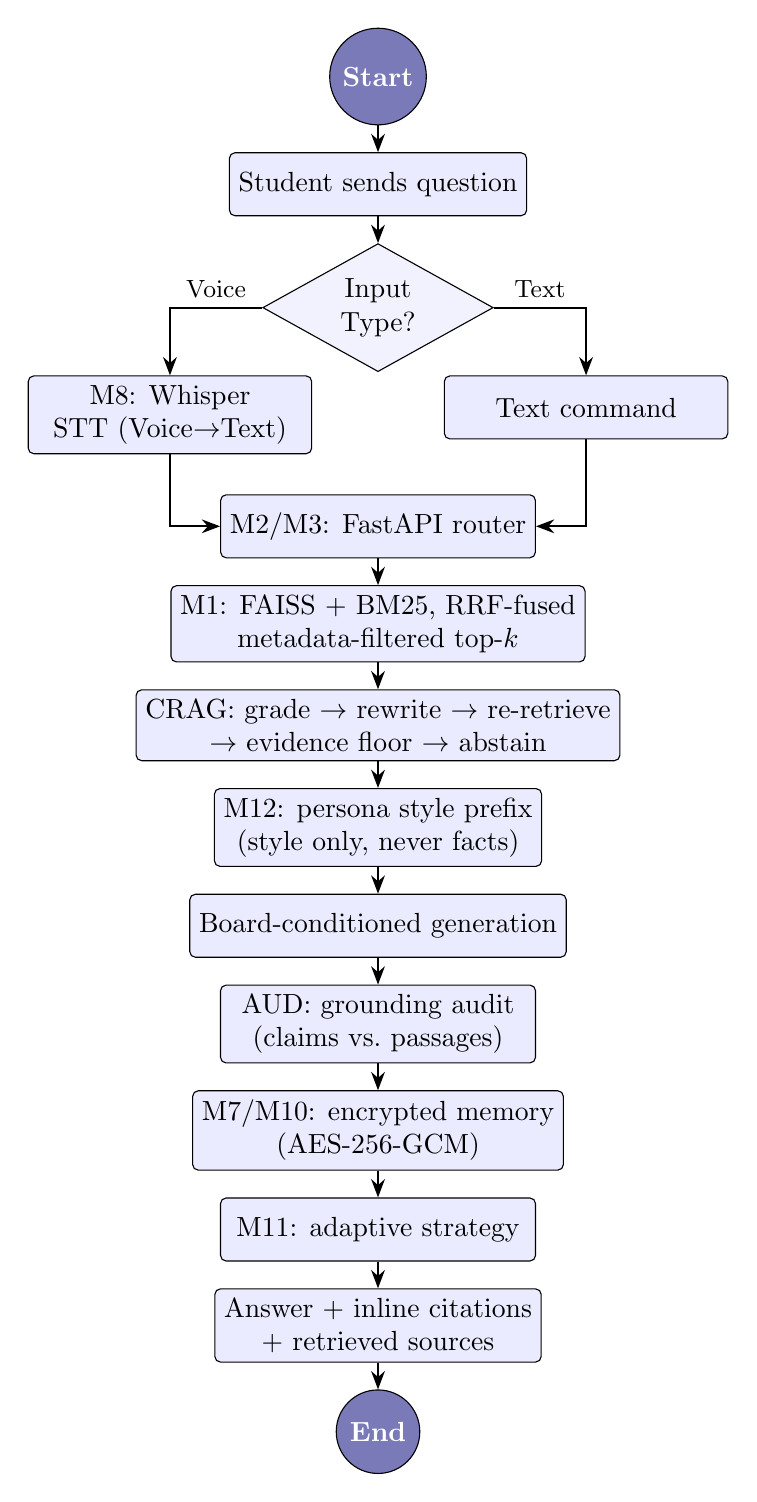
\begin{tikzpicture}[node distance=0.34cm and 0.34cm]
\node[term]  (start)   {Start};
\node[proc,  below=of start]  (send) {Student sends question};
\node[dec,   below=of send]   (intype)  {Input\\Type?};
\node[proc,  below left=0.45cm and 0.1cm of intype]  (whisper)
      {M8: Whisper\\STT (Voice$\to$Text)};
\node[proc,  below right=0.45cm and 0.1cm of intype] (textrcv)
      {Text command};
\node[proc,  below=1.55cm of intype] (fastapi) {M2/M3: FastAPI router};
\node[procW, below=of fastapi] (datapipe)
      {M1: FAISS + BM25, RRF-fused\\metadata-filtered top-$k$};
\node[procW, below=of datapipe] (crag)
      {CRAG: grade $\to$ rewrite $\to$ re-retrieve\\$\to$ evidence floor $\to$ abstain};
\node[procW, below=of crag] (persona)
      {M12: persona style prefix\\(style only, never facts)};
\node[procW, below=of persona]  (llm)
      {Board-conditioned generation};
\node[procW, below=of llm]      (audit)
      {AUD: grounding audit\\(claims vs.\ passages)};
\node[procW, below=of audit]    (memsec)
      {M7/M10: encrypted memory\\(AES-256-GCM)};
\node[procW, below=of memsec]   (adapt) {M11: adaptive strategy};
\node[proc,  below=of adapt] (deliver)
      {Answer + inline citations\\+ retrieved sources};
\node[term,  below=of deliver] (endnode) {End};
\draw[arr] (start)   -- (send);
\draw[arr] (send)    -- (intype);
\draw[arr] (intype)  -| node[near start,above,font=\small]{Voice} (whisper);
\draw[arr] (intype)  -| node[near start,above,font=\small]{Text}  (textrcv);
\draw[arr] (whisper) |- (fastapi);
\draw[arr] (textrcv) |- (fastapi);
\draw[arr] (fastapi) -- (datapipe);
\draw[arr] (datapipe)-- (crag);
\draw[arr] (crag)    -- (persona);
\draw[arr] (persona) -- (llm);
\draw[arr] (llm)     -- (audit);
\draw[arr] (audit)   -- (memsec);
\draw[arr] (memsec)  -- (adapt);
\draw[arr] (adapt)   -- (deliver);
\draw[arr] (deliver) -- (endnode);
\end{tikzpicture}%
}
\caption{End-to-end request lifecycle. Retrieval is metadata-filtered by
subject, level and board before the corrective layer grades it, and the
generated answer is audited against the passages that produced it before
delivery.}
\label{fig:flowchart}
\end{figure}

\subsection{Data Pipeline and Retrieval}
The corpus comprises Pre-University textbooks and board question papers for
physics, chemistry, mathematics and biology across both years, chunked at $500$
tokens with $50$-token overlap and encoded with
\texttt{all-MiniLM-L6-v2} into a FAISS inner-product index of
$7{,}668$ passages. Curating clean source material matters as much as the model
itself, a point stressed in data-collection practice for machine
learning~\cite{roh2021}. Every query is filtered by subject, level, board and
document type before ranking, and passages scoring below a cosine threshold of
$0.30$ are discarded.

\subsection{Lexical Fusion}
\label{sec:hybrid}
A $384$-dimensional sentence embedding is a lossy summary. It generalises, which
is what makes semantic search work, but the same compression blurs exactly the
rare tokens that carry most of the meaning in a science syllabus: \emph{Snell},
\emph{Le Chatelier} and \emph{sigma bond} all sit near their topical
neighbourhood, so a query naming one can rank a passage that merely discusses
the surrounding topic above the passage that defines it.

We therefore add a BM25 arm~\cite{robertson2009} ($k_1=1.5$, $b=0.75$) over the
same chunk metadata and fuse the two rankings by reciprocal rank
fusion~\cite{cormack2009}, $\sum_r 1/(k + \text{rank}_r)$ with $k=60$. Fusing \emph{positions} rather than scores avoids having to make a
cosine of $0.42$ commensurate with a BM25 score of $11.3$. The lexical index is
built lazily over the $7{,}669$ stored passages ($48{,}010$ terms, $0.8$\,s) and
rebuilt when the corpus grows. Because the dense index is flat inner-product,
a lexical-only hit can be given its true cosine by reconstructing its stored
vector, so the downstream similarity floor applies to both arms rather than
admitting lexical hits unscored. Section~\ref{sec:hybrideval} measures the
effect.

\subsection{Corrective Retrieval Layer}
\label{sec:crag}
Each surviving passage is graded by a language model on a three-point scale
(fully supports / background only / unrelated or front matter). If the best
grade reaches $0.90$ the graded passages are used; otherwise the query is
rewritten into textbook vocabulary, retrieval repeated and the results merged,
and if nothing usable survives the system declines. Passages below $0.50$ are
dropped, and a content-based filter removes publisher front matter before
grading at negligible cost.

\subsubsection{Evidence Floor}
\label{sec:floor}
Table~\ref{tab:ablation} attributed the $3$B grader's eleven false refusals to
grader capacity. Instrumenting the loop locates the mechanism more precisely:
the grader does not merely misrank, it returns $0.0$ for \emph{every} retrieved
passage on questions plainly in syllabus, leaving the generator with one
passage or none --- and a generator given almost no evidence does not abstain,
it falls back on parametric memory, the very failure the layer exists to
prevent.

We therefore add a floor. When grading leaves fewer than $n=3$ passages but
retrieval returned candidates the dense index puts plainly on topic, those are
restored in retrieval order. The restoration bar is a higher similarity than
the one admitting a passage for grading, because two cases must be told apart:
a harsh grader rejecting relevant passages, and a grader correctly rejecting
irrelevant ones. Similarity separates them only partly, so the bar is a tuned
operating point. Over the benchmark the top-1 cosine for an answerable question
has median $0.602$ (range $0.234$--$0.957$) against $0.306$ ($0.201$--$0.650$)
out of syllabus: the distributions overlap and no threshold divides them.
Sweeping it trades the errors directly --- at $0.40$, eleven of $150$ answerable
questions fall below and seven of $24$ out-of-syllabus rise above; at the
chosen $0.45$, seventeen and four; at $0.50$, twenty-nine and two. Abstention
is not bypassed: when nothing clears the admission threshold there is nothing
to restore.

\subsection{Board-Conditioned Generation}
\label{sec:diagram}
Interpolating a board name into a prompt conveys nothing, so each board carries
its conventions explicitly. Karnataka Pre-University uses a $1/2/3/5$-mark
structure where five-mark items expect a derivation, labelled diagram or
numerical and marks are awarded per visible step; CBSE uses a stepwise
value-point scheme where each point must appear separately. Answers follow the
shape the marking scheme rewards --- direct answer, explanation in textbook
terminology, governing formula with symbols and SI units, then a worked example
--- and cite evidence inline, stating which part of a question the retrieved
material does not cover rather than filling it from memory.

The module also renders a retrieved topic as one of five diagram forms, since
Karnataka five-mark items often ask for a labelled diagram. Each form is pinned
to a single Mermaid grammar, because a grammar chosen per request is one the
validator cannot check. The difficulty is parsing rather than generation:
models write plausible but invalid Mermaid, and rejecting it wastes a
generation while forwarding it shows a parser error. The module therefore
parses the output into nodes and edges, discards what it cannot interpret and
\emph{re-emits} the diagram, so a malformed label degrades into a cleaned one
rather than a broken render. Nodes come only from retrieved passages, styling
and scripting directives are dropped, and when too little structure survives
the system abstains. Reliability and pedagogical quality are both unevaluated
(§\ref{sec:limits}).

\subsection{Post-Generation Grounding Audit}
\label{sec:audit}
Every requirement above is advisory, and Section~\ref{sec:faithfulness} shows
the cost: handed correct passages, the $3$B model wrote Snell's law, which was
not among them. A citation cannot be enforced by repeating the instruction, but
it is a \emph{claim} about grounding and can be checked mechanically. Checking
output against evidence is the premise of zero-resource hallucination
detection~\cite{manakul2023}; here the evidence is fixed by retrieval rather
than sampled from the model, in the spirit of attribution
evaluation~\cite{gao2023}.

The audit separates three failures a student cannot tell apart:
\textbf{unsupported}, matching no retrieved passage; \textbf{miscited},
supported but not by the passage whose number it carries; and
\textbf{dangling}, citing a passage never retrieved. Checkable sentences are
tokenised against the cited passages and the whole retrieved set; token overlap
is a weak proxy both ways, so it decides only \emph{what to examine}, and
flagged claims then go to a model for an entailment verdict in one batched
call. The auditor tokenises differently from the retrieval arm of
Section~\ref{sec:hybrid}: BM25 discards single-character tokens as noise, but
$v$, $u$, $f$ and $n_1$ are exactly what can be wrong in a physics claim ---
under the retrieval tokeniser the lens-formula sentence fell to four content
words and was skipped. Two numbers are reported separately, claims found
anywhere in the evidence and claims citing the passage carrying them, because
collapsing them yields a headline contradicting its own detail. The answer is
never silently rewritten; a caveat is appended and the structured report
appears beside it (Fig.~\ref{fig:r-grounding}).

\subsection{Adaptive Pedagogical Layer}
\label{sec:adaptive}
A reviewer asked us to define the adaptation rules rather than describe them.
The strategy is selected deterministically from the learner record:
\begin{equation}
s =
\begin{cases}
\textsf{step\_by\_step} & \text{if } \sigma_t < 50\\
\textsf{worked\_example} & \text{else if } c \geq 2\\
\textsf{socratic} & \text{else if } \sigma_t \geq 80\\
\textsf{concise} & \text{otherwise}
\end{cases}
\end{equation}
where $\sigma_t$ is the learner's most recent self-reported percentage on topic
$t$ and $c$ is the number of clarification requests detected in the last ten
dialogue turns. We have \emph{not} evaluated whether this rule improves learning
outcomes; that requires the controlled study described in §\ref{sec:future}.

\subsection{Mock Paper Generation}
For a $70$-mark paper the blueprint produces $15$ slots --- one $2$-mark, one
$3$-mark and thirteen $5$-mark items --- with one internal choice, and assigns a
Bloom level per slot ascending with marks. A structural validator rejects wrong
question counts, blueprint mismatches on identifier, marks or Bloom level,
missing fields, duplicate questions and malformed internal choices, retrying once
before failing. Retrieval for this module is seeded from recurring PYQ topics
rather than the subject name; before this change, every generated question
concerned the textbook's own structure rather than its physics.

\subsection{Persona Engine}
\label{sec:persona}
Fig.~\ref{fig:persona} shows the persona pipeline that a reviewer asked us to
diagram. Registration fetches captions, splits them into $300$-token windows,
encodes and stores them encrypted, then samples thirty passages to distil a
five-field style descriptor, cached once. At inference the question is embedded
and compared against the stored passages; styling is applied only if at least
five passages clear a cosine threshold of $0.30$, and the top three are injected
as a prefix that is explicitly marked untrusted, scoped to phrasing, and
forbidden from contributing facts or implying endorsement.

\begin{figure}[!t]
\centering
\resizebox{0.86\columnwidth}{!}{%
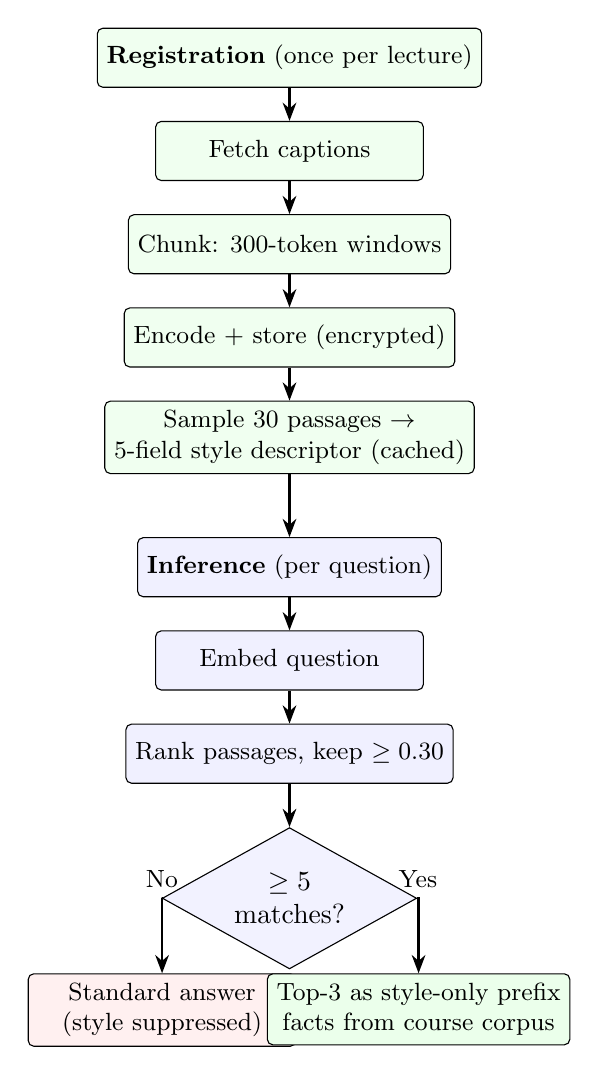
\begin{tikzpicture}[node distance=0.42cm]
\node[stage] (reg) {\textbf{Registration} (once per lecture)};
\node[stage, below=of reg] (fetch) {Fetch captions};
\node[stage, below=of fetch] (chunk) {Chunk: 300-token windows};
\node[stage, below=of chunk] (embed) {Encode + store (encrypted)};
\node[stage, below=of embed] (fp) {Sample 30 passages $\to$\\5-field style descriptor (cached)};
\node[stage, below=0.8cm of fp, fill=blue!6] (inf) {\textbf{Inference} (per question)};
\node[stage, below=of inf, fill=blue!6] (q) {Embed question};
\node[stage, below=of q, fill=blue!6] (rank) {Rank passages, keep $\geq 0.30$};
\node[dec, below=0.55cm of rank] (gate) {$\geq 5$\\matches?};
\node[stage, below left=0.5cm and -0.9cm of gate, fill=red!6] (fallback)
      {Standard answer\\(style suppressed)};
\node[stage, below right=0.5cm and -1.1cm of gate, fill=green!8] (apply)
      {Top-3 as style-only prefix\\facts from course corpus};
\draw[arr] (reg)--(fetch); \draw[arr] (fetch)--(chunk);
\draw[arr] (chunk)--(embed); \draw[arr] (embed)--(fp);
\draw[arr] (fp)--(inf); \draw[arr] (inf)--(q);
\draw[arr] (q)--(rank); \draw[arr] (rank)--(gate);
\draw[arr] (gate) -| node[near start,above,font=\small]{No} (fallback);
\draw[arr] (gate) -| node[near start,above,font=\small]{Yes} (apply);
\end{tikzpicture}%
}
\caption{Persona engine: ingestion, fingerprinting, retrieval and gated
generation. Styling is suppressed unless five transcript passages clear the
relevance floor.}
\label{fig:persona}
\end{figure}

\subsection{Security, Retention, and Data Protection}
\label{sec:security}
Two reviewers identified a contradiction between a ``ten most recent turns''
dialogue memory and a claim of ``session-scoped retention.'' Both statements
were imprecise. The delivered behaviour is:

\begin{itemize}
\item \textbf{Context window.} The ten most recent turns are supplied to the
model as conversational context. This is a prompt-construction limit, not a
retention policy.
\item \textbf{Retention.} Stored records are purged after a configurable
retention period, $30$ days by default.
\item \textbf{Deletion.} A student-invoked endpoint erases the learner record
immediately and returns confirmation.
\item \textbf{At rest.} Stored content is encrypted with AES-256-GCM; learner
identifiers are HMAC-SHA256 pseudonyms, so records are not keyed by a raw
account identifier.
\item \textbf{Access control.} Teacher analytics are gated behind a server-held
key and return aggregate counts, not individual transcripts.
\end{itemize}

We also withdraw an incorrect claim. The submitted version stated that Telegram
delivery provides end-to-end encryption. It does not: MTProto secures the
client--server link, and messages to a bot are readable by the bot platform.
Transport is encrypted in transit, but \emph{not} end-to-end, and we no longer
list end-to-end encryption as a property of the system.

\subsection{Ethical Considerations for Persona Conditioning}
\label{sec:ethics}
A reviewer asked us to address consent, copyright and attribution. The engine
stores a derived five-field style descriptor and short caption excerpts, not
redistributed lecture content, and shows those excerpts as timestamped links
back to the original video, so attribution is preserved and traffic returns to
the creator. The prompt forbids claiming to be the educator or implying
endorsement. Even so, imitating an identifiable person's manner of speaking
without permission raises an objection no technical safeguard dissolves. We
therefore recommend restricting registration to educators who have opted in ---
an institution's own faculty registering their own lectures, which is also the
deployment we consider most useful --- and regard unconsented imitation of a
third-party creator as outside the intended use of this system.

%------------------------------------------------
\section{Benchmark}
%------------------------------------------------
To replace targets with measurements we built a curriculum QA benchmark of
$174$ items: $150$ questions taken verbatim from Karnataka Pre-University board
papers across four subjects and both years ($20$ per cell, except mathematics
at $15$ where symbol-heavy extraction reduced the yield), and $24$ authored
degree-level questions outside the syllabus that must be refused. Nothing in
the answerable split is synthetic.

Gold answers and mark-scheme value points are deliberately left for
subject-teacher annotation: a benchmark whose reference answers were written by
the model family under evaluation would be worthless. The paper therefore
reports \emph{abstention, retrieval economy, citation behaviour and latency},
measurable without gold answers, and not answer correctness, which is not.

%------------------------------------------------
\section{Evaluation}
%------------------------------------------------
\subsection{Hardware and Measured Throughput}
\label{sec:latency}
The submitted version asserted sub-five-second latency for a $7$B model on an
AWS EC2 t3.medium instance. Reviewers correctly identified this as unjustified.
We withdraw it and report measurements from the development host: a $4$-core
AMD Ryzen~5 7235HS with $11.7$\,GiB RAM and an RTX~3050 laptop GPU with
$4.0$\,GiB VRAM. Table~\ref{tab:throughput} gives measured decode throughput.

\begin{table}[htbp]
\caption{Measured generation throughput. A 4-bit $7$B model needs
$\approx 4.7$\,GiB and cannot be resident in $4.0$\,GiB of VRAM.}
\label{tab:throughput}
\centering
\begin{tabular}{llr}
\toprule
\textbf{Model} & \textbf{Placement} & \textbf{Tokens/s} \\
\midrule
Qwen2.5-7B & CPU only (CUDA unavailable) & 4.7 \\
Qwen2.5-3B & CPU only (CUDA unavailable) & 5.0 \\
Qwen2.5-7B & 62\%/38\% CPU/GPU & 6.5 \\
Qwen2.5-3B & 79\% GPU & \textbf{19.6} \\
\bottomrule
\end{tabular}
\end{table}

Two consequences follow. The sub-five-second target is attainable only for
short tutoring answers, not for practice-paper generation, where a $70$-mark
paper expands to several thousand tokens in one request. And model choice is a
\emph{capability} decision, not only a speed one: the $3$B model is four times
faster but could not emit a blueprint-conforming paper at all.

A reviewer asked for latency split into retrieval and generation. Over forty
benchmark questions on the same host, retrieval costs a median $30$\,ms in
total --- $18$\,ms to encode the query, $2$\,ms for the dense search over all
$7{,}669$ passages, $9$\,ms for the BM25 arm, $0.1$\,ms to fuse them --- with a
$95$th percentile of $54$\,ms; only a process's first query pays more, for the
one-off encoder load. Against the $13$--$15$\,s end-to-end figures of
Tables~\ref{tab:ablation} and~\ref{tab:floor} that is under half a percent of a
request. Latency \emph{is} generation here, which is also why the corrective
layer's extra grading passes dominate the cost it adds.

\subsection{Lexical Fusion and Exact-Term Recall}
\label{sec:hybrideval}
Relevance is not annotated in our benchmark, so we do not claim to measure it.
We measure the narrow property a lexical arm is supposed to repair, under an
explicit proxy: for each of the $150$ answerable questions we take its rarest
content word by document frequency in the index --- the token a dense encoder is
most likely to blur --- and ask at what rank the first retrieved passage
containing that token appears, over the top five.

Dense retrieval alone reaches that passage within the top five for $91$ of
$150$ questions at $\mathrm{MRR} = 0.493$; with the lexical arm fused in, $100$
of $150$ at $0.566$. Question by question, fusion is better on $32$, worse on
$3$, identical on $115$ --- an asymmetry that matters more than the mean, since
fusion rarely displaces a good dense result and usually improves the ranking it
does change.

Two cautions. This is exact-term recall, not relevance: a passage can hold the
rare token without answering the question, so the gain is not an answer-quality
gain. And the effect is invisible at small scale --- on fourteen hand-chosen
rare-term queries the configurations were indistinguishable, and we first
concluded fusion was not worth its cost. That was an artefact of a sample we
chose ourselves, recorded here because a reviewer spot-checking a few queries
will reproduce the null result rather than the measured one.

\subsection{Ablation of the Corrective Layer}
\label{sec:ablation}
Table~\ref{tab:ablation} reports $48$ items per configuration ($40$ answerable,
$8$ out-of-syllabus). Abstention precision is the share of refusals that were
correct; recall is the share of out-of-syllabus questions refused.

\textit{Scope note.} The items are the first in benchmark order rather than a
stratified sample, and because the benchmark is assembled subject by subject,
all $40$ answerable items are \emph{physics}. The ablation characterises one
subject, not the whole benchmark, and subject-level generalisation is not
established; a stratified re-run is the obvious next step and the released
driver supports it.

\begin{table}[htbp]
\caption{Ablation of the corrective retrieval layer, $48$ items per
configuration drawn from the physics split (see scope note).
\emph{Src.} is the mean number of cited source references per response,
averaged over all items including refusals.}
\label{tab:ablation}
\centering
\begin{tabular}{lrrrrr}
\toprule
\textbf{Configuration} & \textbf{Src.} & \textbf{Abst.\,P} & \textbf{Abst.\,R} & \textbf{False} & \textbf{Lat.\,(s)} \\
\midrule
Vanilla RAG              & 4.90 & \textbf{1.00} & 0.62 & \textbf{0}  & 13.3 \\
+ boilerplate filter     & 4.81 & \textbf{1.00} & 0.62 & \textbf{0}  & 14.0 \\
+ CRAG ($3$B grader)     & 1.08 & 0.42 & \textbf{1.00} & 11 & \textbf{11.5} \\
+ filter + CRAG ($3$B)   & 1.08 & 0.53 & \textbf{1.00} & 7  & 11.8 \\
+ filter + CRAG (strong) & 4.46 & 0.83 & 0.62 & 1  & 17.1 \\
\bottomrule
\end{tabular}
\end{table}

The result does not support the configuration we first built. With a $3$B
grader the layer refuses eleven of forty answerable questions, rejecting all
five retrieved passages for questions plainly in syllabus. Recall reaches
$1.00$ only because the system has become indiscriminately reluctant, while
precision collapses from $1.00$ to $0.42$ and cited sources fall from $4.90$ to
$1.08$ --- partly because refusals cite nothing, so that figure indicates
grounding rather than context size. Replacing only the grader isolates the
cause: sources recover to $4.46$ and false abstentions fall from seven to one,
so the failure lies in grader capacity, not the loop. The corrected system
still does not beat the plain baseline --- recall returns to $0.62$ while
latency rises $29\%$ to $17.1$\,s --- and the boilerplate filter matches vanilla
retrieval on every abstention measure.

Two conclusions follow. An LLM-graded loop is bounded by its grader and below
some threshold is actively harmful, silently turning a working assistant into
one refusing a quarter of legitimate questions. And on curriculum QA already
filtered by subject, level and board, the corrective machinery is not where the
remaining error lies.

\subsubsection{Repairing the Weak Grader}
\label{sec:flooreval}
Is the harm intrinsic to a small grader, or is it the \emph{starvation} harsh
grading produces? Table~\ref{tab:floor} answers it. Adding the evidence floor
of Section~\ref{sec:floor} to the same $3$B grader cuts false abstentions from
eight to two of forty, lifts precision from $0.47$ to $0.78$ and sources from
$1.02$ to $2.56$, while abstention recall is unchanged at $0.88$: the
out-of-syllabus split is refused exactly as often. A mean of $1.33$ restored
passages shows modest work, not wholesale override.

Against the strong grader of Table~\ref{tab:ablation}, which costs a second
model, the floor reaches comparable precision ($0.78$ against $0.83$) with
\emph{better} recall ($0.88$ against $0.62$) and lower latency ($14.7$ against
$17.1$\,s), using only the small grader and a similarity comparison. We revise
the first conclusion rather than withdraw it: a weak grader is harmful, but the
harm is a starved generator rather than mistaken ranking, and it is repairable
without a stronger judge.

\begin{table}[htbp]
\caption{Effect of the evidence floor, $48$ items per configuration from the
physics split. Both rows were measured in the same session; the baseline is
a re-run of the shipped configuration of Table~\ref{tab:ablation} rather than
its published numbers, because generation is sampled and the two differ
slightly. \emph{Rest.} is the mean number of passages restored past the
grader per request.}
\label{tab:floor}
\centering
\begin{tabular}{lrrrrrr}
\toprule
\textbf{Configuration} & \textbf{Src.} & \textbf{Abst.\,P} & \textbf{Abst.\,R} & \textbf{False} & \textbf{Rest.} & \textbf{Lat.\,(s)} \\
\midrule
filter\,+\,CRAG ($3$B) & 1.02 & 0.47 & 0.88 & 8 & 0.00 & 13.1 \\
\quad +\,evidence floor & 2.56 & 0.78 & 0.88 & 2 & 1.33 & 14.7 \\
\bottomrule
\end{tabular}
\end{table}

\subsection{Generator Capacity and Faithfulness}
\label{sec:faithfulness}
Holding retrieval fixed, we compared a local $3$B model against a substantially
stronger model on identical retrieved passages. Asked to derive $F = ma$, the
local model produced Snell's law of refraction --- correct physics, but
\emph{absent from the retrieved context}. Given the same five passages, the
stronger model stated that the derivation was not present in the supplied
material and declined that part of the question.

This is the central reliability finding. Retrieval gating and abstention are
enforced in code and hold regardless of model. Everything downstream of ``the
model is now generating'' --- grounding instructions, citation requirements,
partial-coverage admissions --- is advisory, and a small model does not reliably
obey it. An architecture's faithfulness guarantees are therefore bounded by the
instruction-following capacity of its generator, which we believe deserves more
attention than it receives in system papers.

\subsection{Grounding Audit}
\label{sec:groundingeval}
Section~\ref{sec:faithfulness} gave one case; the audit puts a number on it.
Over the same $48$ items the shipped configuration answered $37$ of the $40$
answerable questions, and the audit read back $8.1$ claims per answer, roughly
$300$ checkable statements.

Two quantities separate sharply: a mean $0.781$ of an answer's claims are
traceable to the retrieved passages, but only $0.065$ cite the passage carrying
them. The model mostly writes from the material it was given and almost never
says which part --- different failures with different remedies, and either
reported alone would mislead. Twenty-eight of the $37$ answers ($76\%$) contain
at least one untraceable statement, the measured frequency of the failure
Section~\ref{sec:faithfulness} showed once. No answer cited a passage never
retrieved, which is a consequence of the low citation rate rather than a
success. The audit costs $14.5$\,s per request against $14.7$\,s without it
(Table~\ref{tab:floor}), inside run-to-run variation, because the lexical pass
is free and the entailment pass runs once over only the flagged claims. Its
\emph{accuracy}, as distinct from its cost, is unvalidated (§\ref{sec:limits}).

\subsection{Judged Answer Quality, and Whether the Judge Can Be Trusted}
\label{sec:judged}
Reviewers asked for RAGAS-style scores. We report them, and why a single such
score should not be relied on.

Twenty-two answered benchmark items were scored twice over \emph{identical}
answers, by Qwen2.5-7B --- the generator's own family --- and by Gemini 2.5
Flash from another. Faithfulness follows the RAGAS definition: decompose the
answer into statements, count those inferrable from the retrieved context.
Relevancy is a direct judge rating, not RAGAS's question-regeneration
procedure, and is labelled as such. Table~\ref{tab:judged} gives both columns.

The judges disagree. Their faithfulness scores correlate at $r = -0.074$ --- no
relationship --- with mean absolute difference $0.288$, agreeing on only $59\%$
of items to within $0.25$. Much of the gap is mechanical: Gemini decomposes an
answer into $8.1$ statements where Qwen finds $4.3$, so the denominators differ
by a factor of two. The rest is judgement; on the binary PSC labels agreement
is $\kappa = 0.182$, barely above chance.

We draw the conclusion the numbers support rather than the one we wanted.
Reviewer~1 asked us to mitigate judge circularity by separating judge from
generator; we did, and found the separation does not stabilise the measurement.
A faithfulness figure from one judge is a property of that judge as much as of
the system, so we report the pair and the spread rather than a headline value.
This also argues that lexical auditing and abstention --- mechanisms needing no
judge --- deserve more weight than judged scores in systems of this kind.

\begin{table}[htbp]
\caption{Judged evaluation of the same $22$ answers and $9$ persona answers by two judges: Qwen2.5-7B, from the generator\textquotesingle{}s own family, and Gemini 2.5 Flash from another. The generator is Qwen2.5-3B throughout, so the columns differ only in who is scoring. Faithfulness follows the RAGAS definition; relevancy is a direct judge rating, not RAGAS\textquotesingle{}s question-regeneration procedure.}
\label{tab:judged}
\centering
\begin{tabular}{lrr}
\toprule
\textbf{Measure} & \textbf{Qwen2.5-7B} & \textbf{Gemini 2.5} \\
\midrule
Faithfulness (RAGAS definition) & 0.676 & 0.537 \\
Statements extracted per answer & 4.3 & 8.1 \\
Answer relevancy (judge-rated) & 0.784 & 0.832 \\
PSC (submitted target $0.78$) & 0.222 & 0.333 \\
\midrule
\multicolumn{3}{l}{\emph{Agreement between the two judges}} \\
Faithfulness correlation ($r$) & \multicolumn{2}{r}{-0.074} \\
Mean absolute difference & \multicolumn{2}{r}{0.288} \\
PSC agreement ($\kappa$) & \multicolumn{2}{r}{0.182} \\
\bottomrule
\end{tabular}
\end{table}

\subsection{Persona Style Consistency, Measured}
\label{sec:pscval}
The submitted version proposed PSC with a $0.78$ target and a threshold we
withdrew as uncalibrated. We now measure it as defined: the judge sees a
persona-conditioned answer, three genuine excerpts from the registered educator
and three neutral baseline passages, and labels the answer style-consistent;
PSC is the share judged consistent.

Twelve questions on the registered lecture's topic were used, three from the
benchmark and nine authored, since the benchmark's whole board papers hold only
three well-formed items on electric flux. The persona engaged on nine and was
suppressed on three for want of five matching transcript passages, so the
relevance gate behaves as Section~\ref{sec:persona} describes. PSC is $0.222$
by the same-family judge and $0.333$ by the cross-family one, both far below
$0.78$. The target is not met and we withdraw it rather than restate it as an
aspiration.

Generating persona and standard answers from the \emph{same} passages isolates
the style prefix. Persona conditioning left lexical grounding essentially
unchanged ($0.943 \rightarrow 0.962$), lowered judged faithfulness slightly
under both judges ($0.690 \rightarrow 0.630$ and $0.661 \rightarrow 0.638$),
moved relevancy in opposite directions depending on the judge, and lengthened
answers by about $11\%$. On this evidence persona conditioning is close to
quality-neutral and clearly not style-effective at the level first claimed.

\subsection{System Output}
\label{sec:output}
Figs.~\ref{fig:r-ask}--\ref{fig:r-grounding} show live output from the deployed
system against the index described above, included because two reviewers of the
submitted version observed that it demonstrated no working behaviour.
Fig.~\ref{fig:r-ask} shows a grounded answer with inline citation markers and a
\emph{Retrieved sources} list naming the textbook file and page behind each
one, the verifiability mechanism of Section~\ref{sec:faithfulness}.
Fig.~\ref{fig:r-persona} shows the style descriptor distilled for a registered
educator with its passage count and timestamped source links, supporting the
attribution discussed in Section~\ref{sec:ethics}.
Fig.~\ref{fig:r-grounding} shows the grounding audit on the two-part question
of Section~\ref{sec:faithfulness} and makes that argument visible: six of seven
statements trace to the retrieved passages, but \emph{none} carries a citation
identifying which. The two quantities move independently, which is why they are
reported separately, and each flagged statement is named with its reason rather
than summarised into a score.

\begin{figure}[!t]
\centering

\includegraphics[width=\columnwidth]{figures/r01-ask-result.png}
\caption{Grounded answer with inline citations resolving to textbook file and
page numbers.}
\label{fig:r-ask}
\end{figure}

\begin{figure}[!t]
\centering

\includegraphics[width=\columnwidth]{figures/r07-persona-fingerprint.png}
\caption{Style descriptor distilled from a registered educator's transcript,
with passage count and timestamped source attribution.}
\label{fig:r-persona}
\end{figure}

\begin{figure}[!t]
\centering
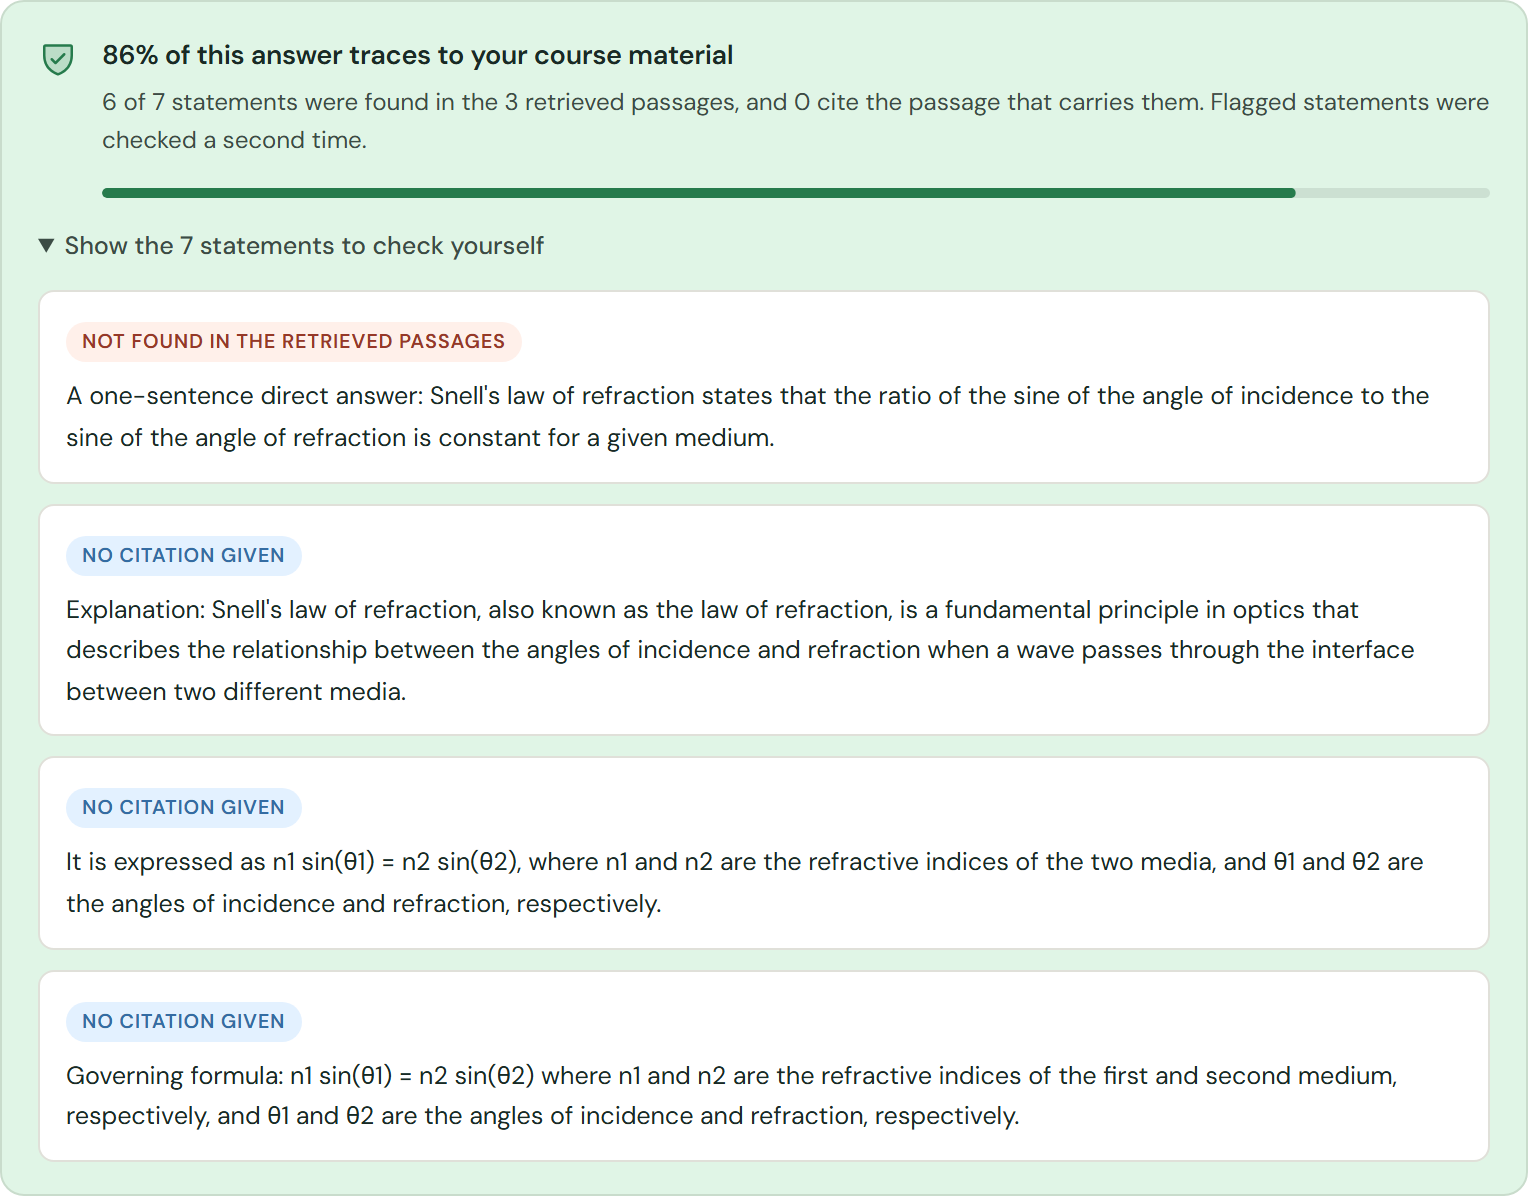
\includegraphics[width=\columnwidth]{figures/r09-grounding-check.png}
\caption{The grounding audit beside an answer. Six of seven statements are
traceable to the retrieved passages while none cites the passage that supports
it, so the two shares are reported separately. Each flagged statement is named
with the reason it was flagged.}
\label{fig:r-grounding}
\end{figure}

\subsection{Persona: Cross-Lingual Limitation and Working Case}
\label{sec:personaeval}
A registered Hindi-caption lecture ($219{,}041$ embedding tokens, truncated to
$89{,}991$ to fit the engine's ceiling, yielding $360$ passages) produced a
correct style descriptor that identified Hindi--English code-switching, Hindi
discourse markers and a step-by-step questioning approach. Yet persona
conditioning never fired. With an English-trained encoder an English question
retrieves the English corpus but matches fewer than five Hindi passages, while a
Hindi question fails the course-evidence gate. The two requirements are mutually
exclusive under a monolingual encoder, and the five-passage floor correctly
suppressed styling rather than faking it.

Registering an English-caption lecture ($8{,}444$ tokens, $34$ passages) on the
same code path produced persona application on the first attempt: three
transcript passages cleared the floor, and the interface displayed the educator
name, the applied-style notice, and timestamped links to the source video under
a heading marking them as teaching-style references rather than factual sources.
Every numbered citation in the answer resolved to the institutional textbook,
with no leakage from the transcript --- the provenance separation held.

This establishes that the pipeline operates and that style and fact provenance
remain separate. It does \emph{not} establish that the text is closer to the
educator's style; Section~\ref{sec:pscval} measures that, and finds it is
largely not.

%------------------------------------------------
\section{What Remains Unmeasured}
\label{sec:limits}
%------------------------------------------------
Reviewers asked for several quantities. Some we now have; the rest we list as
open rather than estimate.

\textbf{PSC is measured; its judges disagree.} The submitted $0.78$ threshold
was described as pilot-calibrated; no pilot was conducted and we withdraw that
claim. Section~\ref{sec:pscval} reports $0.222$ and $0.333$, both far under
target, but the judges agree at only $\kappa = 0.182$, so the direction is
dependable and the value is not. Settling it needs human raters, an inter-rater
statistic, and more than twelve questions.

\textbf{LLM-as-judge circularity is measured, and the news is bad.} Separating
judge from generator by family was our proposed mitigation;
Section~\ref{sec:judged} implements it and finds the judges fail to agree on
identical answers ($r = -0.074$). Family separation removes the
shared-blind-spot objection without delivering a stable measurement, so we no
longer present it as sufficient. Missing is a human-rated calibration subset,
position-swap debiasing and a larger panel; until then we lean on the
mechanisms needing no judge.

\textbf{No faculty validation of correctness.} Judged faithfulness measures
whether an answer follows from the retrieved passages, not whether it is
correct or would earn marks. Faculty annotation of the benchmark's gold answers
is incomplete, so we report no accuracy figure. A model judge is not a
substitute and we do not offer one as such.

\textbf{No Technology Acceptance Model data.} The TAM
instrument~\cite{davis1989} and the $N \geq 30$ cohort were planned, not
executed. TAM records what participants report about a system they have used,
so no simulation can stand in for it; the figure cannot be supplied without
running the study.

\textbf{The grounding audit is unvalidated.} We report how often it flags a
claim, not whether it is right to. Neither false-alarm nor miss rate is known;
establishing them needs a teacher-marked subset of sentences.

\textbf{PYQ topic matching is lexical.} The trend engine ranks single-token
keywords by TF-IDF, does not match differently worded questions expressing one
concept, and its extracted topics include PDF artefacts. No ranking accuracy
has been verified against a teacher-labelled key.

\textbf{Practice papers are validated structurally, not academically.} A
validator enforces question distribution, mark allocation and internal choice,
so format conformance is checked in code. Whether questions meet board
standard, whether an assigned Bloom level matches the question generated, and
whether a paper aligns with learning outcomes are content judgements needing
faculty annotation.

\textbf{Speech coverage is declared, not measured.} The interface accepts eight
languages --- English, Hindi, Kannada, Tamil, Telugu, Malayalam, Marathi,
Bengali --- with Whisper (base) transcribing and synthesis disabled by default.
That is what is accepted, not what is handled well: we have measured word error
rate for none, nor the downstream effect of a transcription error, which
matters more, since a misheard term changes the retrieval query itself.

\textbf{Diagram generation is described, not evaluated.} We report no rate at
which diagrams are drawn, abstained on or repaired, and no judgement of
quality. Re-emission makes output parseable by construction --- a property of
the code, not a measured result.

%------------------------------------------------
\section{Reproducibility}
%------------------------------------------------
The benchmark, the ablation drivers and the table generators are released with
the system. Each ablation restarts the service in every configuration it
reports and writes both Markdown and \LaTeX{}, so Tables~\ref{tab:ablation}
and~\ref{tab:floor} can be regenerated rather than taken on trust, and the
retrieval study behind the threshold sweep runs without a generator at all.
The judged evaluation caches every answer with the passages that produced it,
so a third judge can re-score identical answers without regenerating them.
Because generation is sampled, the evidence-floor rows are measured against a
re-run of the shipped configuration rather than the published numbers, and the
driver runs that baseline first for exactly this reason.
We consider all of this important precisely because our
headline architectural addition did not survive its own ablation.

%------------------------------------------------
\section{Conclusion and Future Work}
\label{sec:future}
%------------------------------------------------
We presented StudyMate, a curriculum-grounded teaching assistant for Karnataka
Pre-University and CBSE students, and measured it rather than projecting it.
Retrieval already filtered by subject, level and board is hard to improve with
a corrective loop: a weak grader is actively harmful, a strong one costs
latency without measurably improving grounding, and a near-zero-cost
boilerplate filter matched both. The harm, though, proved specific and cheap to
fix --- the grader starves the generator rather than misranking for it, and a
similarity-gated evidence floor recovers most of what a strong grader buys
without running one. Grounding is likewise better verified than instructed:
across $300$ audited statements, $78\%$ were traceable to the retrieved
passages while only $6.5\%$ named the passage supporting them. Persona
conditioning works end to end with correct provenance separation, but only when
the encoder spans the languages involved, and against the style metric we
proposed it reaches $0.22$--$0.33$ rather than $0.78$.

The judged evaluation carries a warning we did not anticipate. Separating judge
from generator by model family was our answer to a circularity objection; doing
it revealed that two judges scoring identical answers do not agree, on
faithfulness or on style. The separation removes the objection without
producing a stable number. We therefore weight the parts of this evaluation
that need no judge --- abstention against a held-out split, lexical audits,
retrieval measured directly --- and suggest that a reported LLM-judged
faithfulness figure name its judge with equal prominence.

Three lines of work follow. A multilingual encoder should restore
cross-lingual persona conditioning, the change most likely to help the Hindi-
and Kannada-medium learners the engine was designed for. Teacher annotation of
the released benchmark would convert board-conditioned generation from a design
argument into a measured one --- whether answers written to a board's
convention earn more marks under its scheme, scored blind by practising
examiners --- and would supply the human anchor the judged evaluation lacks.
And abstention deserves first-class treatment, trading against coverage in ways
a single accuracy number hides. Beyond these, federated corpus
sharing~\cite{fajardo2025} would let colleges pool material without
centralising student data.

We note finally that the most useful result in this paper began as a negative
one. We could have presented the corrective layer as an unqualified improvement;
the released ablation script would have contradicted us within minutes.
Reporting the failure instead is what made it legible enough to diagnose, and
the diagnosis is what produced the repair. We prefer the version that is
reproducible.

%------------------------------------------------
\section*{Acknowledgment}
A plagiarism and AI-content similarity report generated with the
conference-recommended tool accompanies this manuscript as supplementary
material. The prose has been authored and revised by the student team.

%------------------------------------------------
\begin{thebibliography}{20}
\bibitem{lewis2020}
P. Lewis et al., ``Retrieval-Augmented Generation for Knowledge-Intensive
NLP Tasks,'' \textit{Adv. Neural Inf. Process. Syst.}, vol. 33,
pp. 9459--9474, 2020.
\bibitem{bloom1984}
B. S. Bloom, ``The 2 Sigma Problem: The Search for Methods of Group
Instruction as Effective as One-to-One Tutoring,'' \textit{Educ.
Researcher}, vol. 13, no. 6, pp. 4--16, 1984.
\bibitem{lauber2025}
A.-M. Lauber, S. Martin, and B. Pampel, ``How Can I Help You? Didactic
Alignment for RAG Chatbots in Education,'' in \textit{Proc. 17th Int.
Conf. Educ. Technol. Comput. (ICETC)}, 2025, pp. 153--158.
\bibitem{teixeira2025}
S. Teixeira, M. Sonkaya, and P. Georgieva, ``RAG Augmented Large
Language Models as a Tool for Education,'' in \textit{Proc. Int. Conf.
Autom. Informatics (ICAI)}, 2025, pp. 769--774.
\bibitem{neumann2025}
A. T. Neumann, Y. Yin, S. Sowe, S. Decker, and M. Jarke,
``An LLM-Driven Chatbot in Higher Education for Databases and
Information Systems,'' \textit{IEEE Trans. Educ.}, vol. 68, no. 1,
pp. 103--112, 2025.
\bibitem{dong2025}
C. Dong, Y. Yuan, K. Chen, S. Cheng, and C. Wen, ``How to Build an
Adaptive AI Tutor for Any Course Using Knowledge Graph-Enhanced
Retrieval-Augmented Generation (KG-RAG),''
\textit{arXiv preprint arXiv:2311.17696}, 2025.
\bibitem{nguyen2025}
L. Nguyen and T. Quan, ``URAG: Implementing a Unified Hybrid RAG for
Precise Answers in University Admission Chatbots,''
\textit{arXiv preprint arXiv:2501.16276}, 2025.
\bibitem{zhao2024}
Z. Zhao, Z. Yin, J. Sun, and P. Hui, ``Embodied AI-Guided Interactive
Digital Teachers for Education,'' in \textit{SIGGRAPH Asia Educators
Forum}, ACM, 2024.
\bibitem{he2025}
S. He, L. Liu, J. Ma, and Y. Lu, ``RAG-X-Driven Construction of an
Intelligent Platform for Teaching Assistance in Higher Education,''
in \textit{Proc. 5th Int. Conf. Educ. Technol. (ICET)}, 2025,
pp. 238--242.
\bibitem{luo2026}
Y. Luo, D. R. Sarkar, R. H. Sangree, and S. Goswami,
``ARIA: Adaptive Retrieval Intelligence Assistant---A Multimodal RAG
Framework for Domain-Specific Engineering Education,''
\textit{arXiv preprint arXiv:2604.06179}, 2026.
\bibitem{koutsiaki2025}
M. E. Koutsiaki et al., ``From Textbook to Talkbot: A Case Study of a
Greek-Language RAG-Based Chatbot in Higher Education,'' in
\textit{Proc. Barcelona Conf. Educ.}, 2025.
\bibitem{gielis2025}
A. Gielis et al., ``Personalized Self-Assessment Tool Using a Telegram
Bot: A Case Study on Data Structures and Algorithms,''
\textit{arXiv preprint arXiv:2601.06225}, 2025.
\bibitem{es2025}
S. Es, J. James, L. Espinosa-Anke, and S. Schockaert,
``RAGAS: Automated Evaluation of Retrieval Augmented Generation,''
\textit{arXiv preprint arXiv:2309.15217}, 2025.
\bibitem{davis1989}
F. D. Davis, ``Perceived Usefulness, Perceived Ease of Use, and User
Acceptance of Information Technology,'' \textit{MIS Quart.}, vol. 13,
no. 3, pp. 319--340, 1989.
\bibitem{roh2021}
Y. Roh, G. Heo, and S. E. Whang, ``A Survey on Data Collection for
Machine Learning: A Big Data--AI Integration Perspective,''
\textit{IEEE Trans. Knowl. Data Eng.}, vol. 33, no. 4,
pp. 1328--1347, 2021.
\bibitem{kuhail2023}
M. A. Kuhail et al., ``Interacting with Educational Chatbots: A
Systematic Review,'' \textit{Educ. Inf. Technol.}, vol. 28, no. 1,
pp. 973--1018, 2023.
\bibitem{wollny2021}
A. Wollny et al., ``Are We There Yet? A Systematic Literature Review on
Chatbots in Education,'' \textit{Front. Artif. Intell.}, vol. 4,
p. 654924, 2021.
\bibitem{fajardo2025}
V. A. Fajardo et al., ``FedRAG: A Framework for Fine-Tuning
Retrieval-Augmented Generation Systems,''
\textit{arXiv preprint arXiv:2506.09200}, 2025.
\bibitem{li2023}
Y. Li et al., ``Style-Conditioned Language Generation for Personalized
Dialogue,'' in \textit{Proc. ACL}, 2023, pp. 4810--4824.
\bibitem{yan2024crag}
S.-Q. Yan, J.-C. Gu, Y. Zhu, and Z.-H. Ling, ``Corrective Retrieval
Augmented Generation,'' \textit{arXiv preprint arXiv:2401.15884}, 2024.
\bibitem{robertson2009}
S. Robertson and H. Zaragoza, ``The Probabilistic Relevance Framework: BM25
and Beyond,'' \textit{Foundations and Trends in Information Retrieval},
vol. 3, no. 4, pp. 333--389, 2009.
\bibitem{cormack2009}
G. V. Cormack, C. L. A. Clarke, and S. B\"{u}ttcher, ``Reciprocal Rank Fusion
Outperforms Condorcet and Individual Rank Learning Methods,'' in
\textit{Proc. 32nd ACM SIGIR}, 2009, pp. 758--759.
\bibitem{manakul2023}
P. Manakul, A. Liusie, and M. J. F. Gales, ``SelfCheckGPT: Zero-Resource
Black-Box Hallucination Detection for Generative Large Language Models,'' in
\textit{Proc. EMNLP}, 2023, pp. 9004--9017.
\bibitem{gao2023}
T. Gao, H. Yen, J. Yu, and D. Chen, ``Enabling Large Language Models to
Generate Text with Citations,'' in \textit{Proc. EMNLP}, 2023,
pp. 6465--6488.
\bibitem{liu2024persona}
Z. Liu, S. X. Yin, G. Lin, and N. F. Chen, ``Personality-Aware Student
Simulation for Conversational Intelligent Tutoring Systems,'' in
\textit{Proc. EMNLP}, 2024, pp. 626--642.
\bibitem{liu2025pace}
H. Liu, Z. Zhang, G. Lin, Y. Jia, and H. Peng, ``One Size Doesn't Fit All: A
Personalized Conversational Tutoring Agent for Mathematics Instruction,''
\textit{arXiv preprint arXiv:2502.12633}, 2025.
\end{thebibliography}
\end{document}
